% 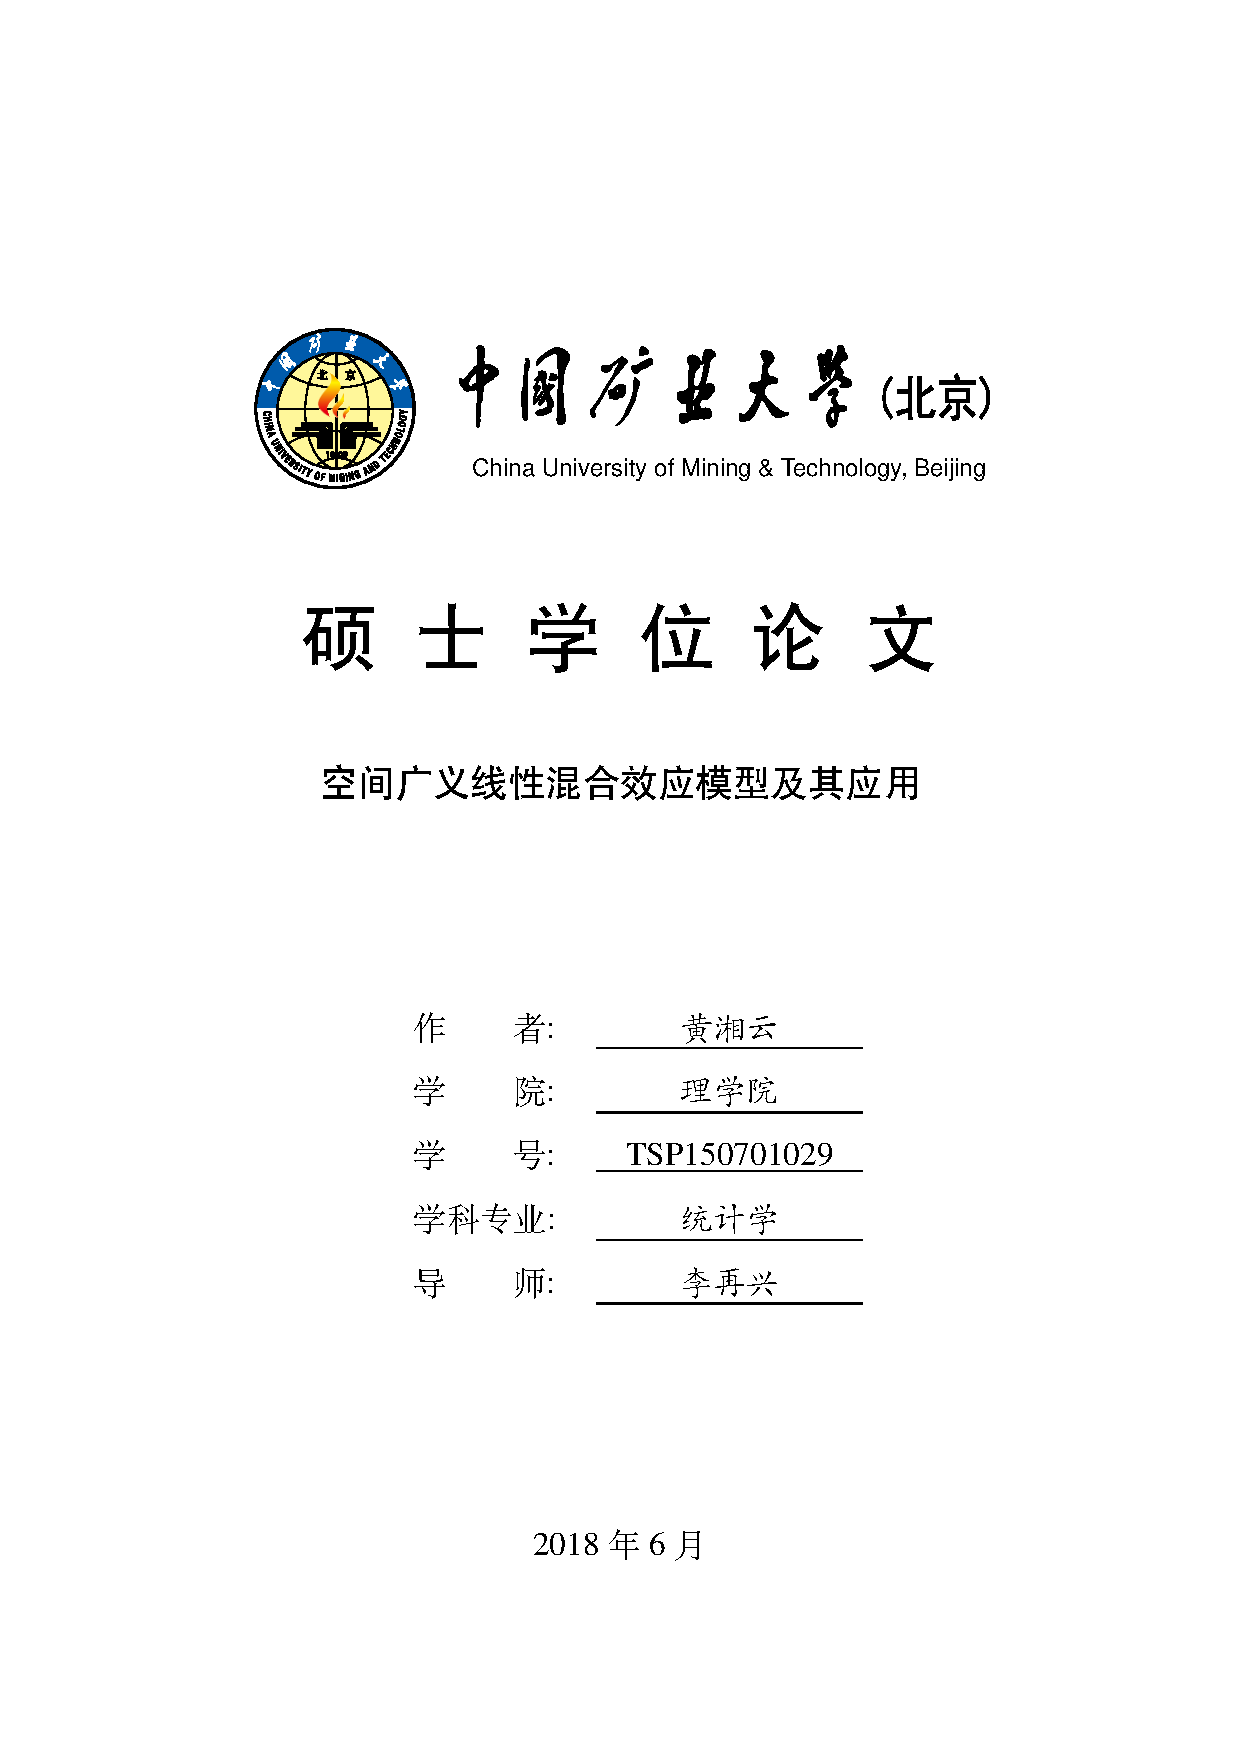
\includepdf[pages=-]{cover.pdf}

%%%%%%%%%%%%%%%%%% 封面 %%%%%%%%%%%%%%%%%%%%%%% 
\thispagestyle{empty}

\begin{figure}[h]
\vspace{1.9cm}
\centering
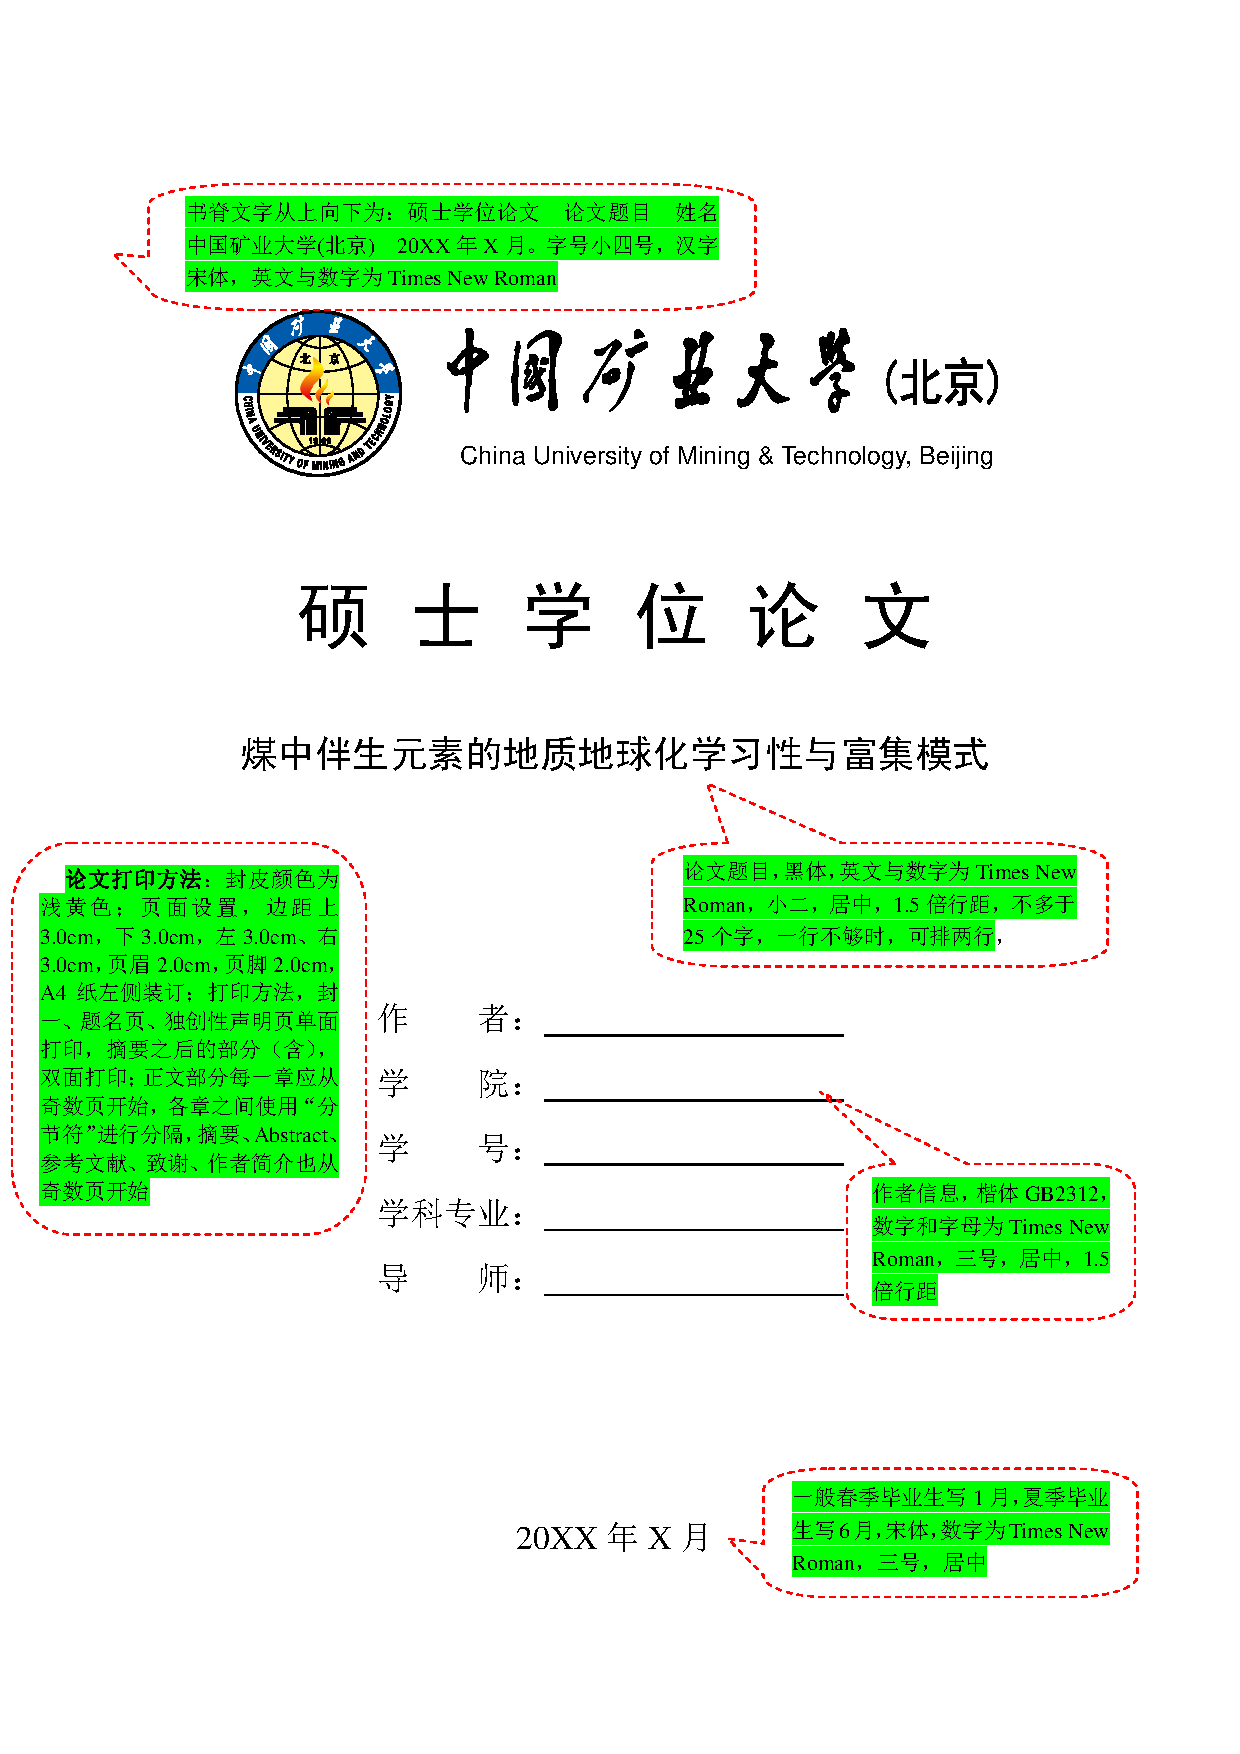
\includegraphics[width=5in]{cumtb}
\end{figure}

\vspace{1cm} % 垂直距离 1.0cm

\begin{center}
{\huge{\heiti\zihao{-0}硕~ 士~ 学~ 位~ 论~ 文}}   \\

\vspace{1.5cm} % 垂直距离 1.5cm

{\heiti\zihao{-2}空间广义线性混合效应模型及其应用} \\ % 论文题目
\end{center}

\vspace{2.5cm}

\begin{flushleft}
\hspace{4cm}\zihao{3}\makebox[0.16\textwidth][s]{作者:} \quad \underline{\makebox[0.3\textwidth][c]{\kaishu 黄湘云}}\\
\vspace{0.2cm}
\hspace{4cm}\zihao{3}\makebox[0.16\textwidth][s]{学院:} \quad \underline{\makebox[0.3\textwidth][c]{\kaishu 理学院}}\\
\vspace{0.2cm}
\hspace{4cm}\zihao{3}\makebox[0.16\textwidth][s]{学号:} \quad \underline{\makebox[0.3\textwidth][c]{TSP150701029}}\\
\vspace{0.2cm}
\hspace{4cm}\zihao{3}\makebox[0.16\textwidth][s]{学科专业:} \quad \underline{\makebox[0.3\textwidth][c]{\kaishu 统计学}}\\
\vspace{0.2cm}
\hspace{4cm}\zihao{3}\makebox[0.16\textwidth][s]{导师:} \quad \underline{\makebox[0.3\textwidth][c]{\kaishu 李再兴}}\\
\end{flushleft}

\vspace{3cm}

\begin{center}
{\songti\zihao{3} 2018 年 6 月} % 日期
\end{center}

%% 空一页
\newpage 
\thispagestyle{empty}
\mbox{} 


\newpage % 新起一页
\thispagestyle{empty}

\begin{flushleft}
\hspace{0.5cm}\makebox[0.18\textwidth][s]{\zihao{4}\songti 中图分类号:}\underline{\makebox[0.2\textwidth][c]{}}
\hspace{1cm}
\hspace{0.5cm}\makebox[0.15\textwidth][s]{\zihao{4}\songti 单位代码:}\underline{\makebox[0.2\textwidth][c]{}}
\vspace{0.2cm}\\
\hspace{0.5cm}\makebox[0.18\textwidth][s]{\zihao{4}\songti 密级:}\underline{\makebox[0.2\textwidth][c]{}}
\end{flushleft}

\vspace{2cm}

\begin{center}
{\heiti\zihao{-1}硕~ 士~ 学~ 位~ 论~ 文}\\
\end{center}

\vspace{1.0cm}

\begin{flushleft}
\hspace{0.5cm}\songti\zihao{4}中文题目:\underline{\makebox[0.75\textwidth][c]{\kaishu 空间广义线性混合效应模型及其应用}} \\
\vspace{0.3cm}
\hspace{0.5cm}\songti\zihao{4}英文题目:\underline{\makebox[0.75\textwidth][c]{Spatial Generalized Linear Mixed Models and }}\\
\vspace{0.3cm}
\hspace{2.7cm}\underline{\makebox[0.75\textwidth][c]{its Applications}}
\end{flushleft}

\vspace*{2.9cm}

\begin{flushleft}
\hspace{0.5cm}\makebox[0.15\textwidth][s]{\songti\zihao{4}作者}:\underline{\makebox[0.2\textwidth][c]{\kaishu 黄湘云}}
\hspace{2.3cm}\makebox[0.15\textwidth][s]{\songti\zihao{4}学号}:\underline{\makebox[0.25\textwidth][c]{\kaishu TSP150701029}}\\
\vspace{0.6cm}

\hspace{0.5cm}\makebox[0.15\textwidth][s]{\songti\zihao{4}学科专业}:\underline{\makebox[0.2\textwidth][c]{\kaishu 统计学}}
\hspace{2.3cm}\makebox[0.15\textwidth][s]{\songti\zihao{4}研究方向}:\underline{\makebox[0.25\textwidth][c]{\kaishu 概率论与数理统计}}\\
\vspace{0.6cm}

\hspace{0.5cm}\makebox[0.15\textwidth][s]{\songti\zihao{4}导师}:\underline{\makebox[0.2\textwidth][c]{\kaishu 李再兴}}
\hspace{2.3cm}\makebox[0.15\textwidth][s]{\songti\zihao{4}职称}:\underline{\makebox[0.25\textwidth][c]{\kaishu 教授}}\\
\vspace{0.6cm}

\hspace{0.5cm}\makebox[0.22\textwidth][s]{\songti\zihao{4}论文提交日期}:\underline{\makebox[0.23\textwidth][c]{\kaishu 2018年5月12日}}
\hspace{0.1cm}\makebox[0.22\textwidth][s]{\songti\zihao{4}论文答辩日期}:\underline{\makebox[0.23\textwidth][c]{\kaishu 2018年5月12日}}\\
\vspace{0.6cm}
\hspace{0.5cm}\makebox[0.22\textwidth][s]{\songti\zihao{4}学位授予日期}:\underline{\makebox[0.23\textwidth][c]{\kaishu 2018年5月12日}}\\
\vspace{0.6cm}
\end{flushleft}

\vspace*{1.5cm}

\begin{center}
{\heiti\zihao{4}中国矿业大学(北京)}
\end{center}

%% 空白页
\newpage 
\thispagestyle{empty}
\mbox{} 

%%%%%%%%%%%%%%%%%%%%% 独创性声明 %%%%%%%%%%%%%%%%%%%%%%%%%%%%%%%%%%%%%
% \chapter*{独创性声明}
\newpage
\thispagestyle{empty}

~~
\vskip 10mm

\begin{center}
\heiti\zihao{3}独创性声明
\end{center}
\vskip 5mm
\par
本人声明所呈交的学位论文是我个人在导师指导下进行的研究工作及取得的研究成果。
尽我所知,除了文中特别加以标注和致谢的地方外,论文中不包含其他人已经发表或撰
写过的研究成果,也不包含为获得中国矿业大学或其他教学机构的学位或证书而使用过的材料。
与我一同工作的同志对本研究所做的任何贡献均已在论文中作了明确的说明并表示谢意。\\
% \vspace{-2.5cm}
\vskip 5mm
\hspace{55mm}作者签名:\underline{\makebox[0.15\textwidth][c]{}}
日期:\underline{\makebox[0.15\textwidth][c]{}} \vskip3mm

\vspace{5.0cm}

\begin{center}
\heiti\zihao{3}关于论文使用授权的说明
\end{center}
\vskip 5mm
\par
本人完全了解中国矿业大学有关保留、使用学位论文的规定,即:学校有权保留送交论文的
复印件,允许论文被查阅或借阅;学校可以公布论文的全部或部分内容,可以采用影印、缩印
或其他复制手段保存论文。
\par
(保密的论文在解密后应遵守此规定) 
\vskip 12mm
\hspace{20mm}作者签名:\underline{\makebox[0.15\textwidth][c]{}}
导师签名:\underline{\makebox[0.15\textwidth][c]{}}
日期:\underline{\makebox[0.15\textwidth][c]{}} \vskip3mm

\thispagestyle{empty}
\mbox{}

%%%%%%%%%%%%%%%%%%%%%%%%% 摘要  %%%%%%%%%%%%%%%%%%%%%%%%%%%%%%%%%%%%%

% 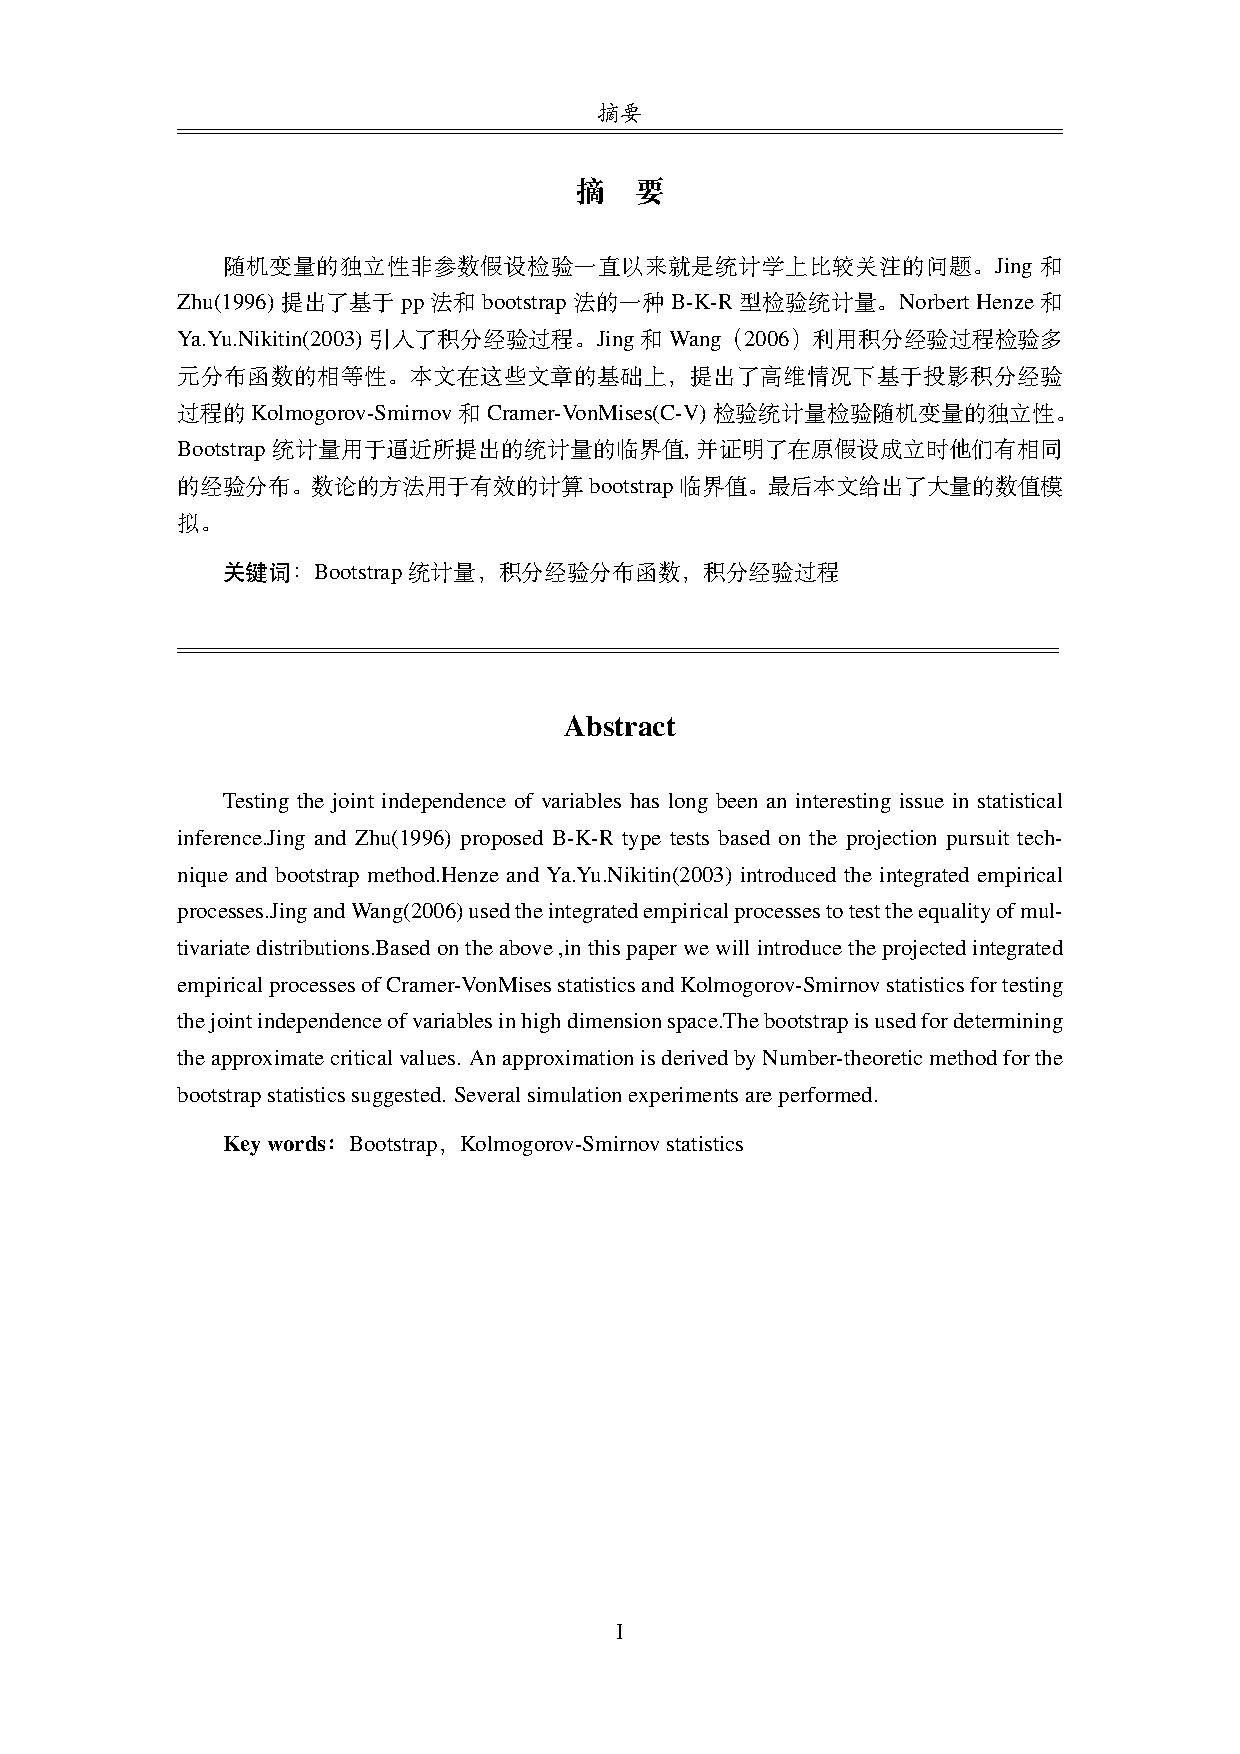
\includepdf[pages=-]{abstract.pdf}

% \newpage
\chapter*{\markboth{摘要}{摘要}{摘\quad 要}}
\pagenumbering{Roman} %
\medskip
随机变量的独立性非参数假设检验一直以来就是统计学上比较关注的问题。Jing 和 Zhu(1996) 提出了基于pp法和bootstrap法的一种B-K-R型检验统计量。Norbert Henze 和 Ya.Yu.Nikitin(2003)引入了积分经验过程。Jing和Wang(2006)利用积分经验过程检验多元分布函数的相等性。本文在这些文章的基础上,提出了高维情况下基于投影积分经验过程的 Kolmogorov-Smirnov 和 Cramer-VonMises(C-V) 检验统计量检验随机变量的独立性。
Bootstrap 统计量用于逼近所提出的统计量的临界值,并证明了在原假设成立时他们有相同的经验分布。
数论的方法用于有效的计算bootstrap临界值。最后本文给出了大量的数值模拟。
\medskip
\par
{\heiti 关键词 :} Bootstrap统计量,积分经验分布函数,积分经验过程

\par
\vspace{1cm}
\noindent\begin{tabular}{l}
\toprule[1pt]\hline
\hspace*{14.5cm}
\end{tabular}

\begin{center}
{\bf \Large Abstract}\\
\vskip 0.6cm
\end{center}
\par
Testing the joint independence of variables has long been an
interesting issue in statistical inference.Jing and Zhu(1996)
proposed  B-K-R type tests based on the projection pursuit technique
and bootstrap method.Henze and Ya.Yu.Nikitin(2003) introduced the
integrated empirical processes.Jing and Wang(2006) used the
integrated empirical processes to test the equality of multivariate
distributions.Based on the above ,in this paper we will introduce
the projected integrated empirical processes of Cramer-VonMises
statistics and Kolmogorov-Smirnov statistics for testing the joint
independence of variables in high dimension space.The bootstrap is
used for determining the approximate critical values. An
approximation is derived by Number-theoretic method for the
bootstrap statistics suggested. Several simulation experiments are
performed.
\medskip
\par

{\bf Key words:} Bootstrap,Kolmogorov-Smirnov statistics

%%% 空一页
\newpage 
\mbox{} 

\addtocontents{toc}{\protect\markboth{目录}{目录}} % 设置页眉处目录
